% !TEX encoding = UTF-8 Unicode
%\chapter{Especificação do QoSPM}
\xchapter{Especificação do QoSPM}{}
\label{cap:especificacao}
\acresetall

	Neste capítulo o QoSPM será especificado, sendo que ele está dividido em quatro seções: na seção 5.1 será descrita a arquitetura do QoSPM; na 5.2 a modelagem do QoSPM através da UML será abordada; na 5.3 será descrito o protocolo utilizado pelos componentes do QoSPM; e para finalizar, a seção 5.4 abordará os principais algoritmos utilizados pelo QoSPM.

\section{Arquitetura do QoSPM}

	A arquitetura do QoSP foi descrita no caítulo \ref{cap:qos_provider}. Agora nós iremos focar a arquitetura do QoSP \textit{Monitoring}. Como foi descrito anteriormente, uma rede com o QoS \textit{Provider} é formada por módulos do QoSP e por roteadores. Além destes elementos, um novo elemento foi adicionado para compor a arquitetura do QoS \textit{Provider}, mas especificadamente do QoSPM, sendo denominado QoSP \textit{Agent} (QoSPA). Para cada roteador existe um módulo do QoSPA, sendo que este tem a função de monitorar o roteador que está vinculado ao mesmo (Figura \ref{fig:arquitetura_qosp}).
	
\begin{figure}
\centering
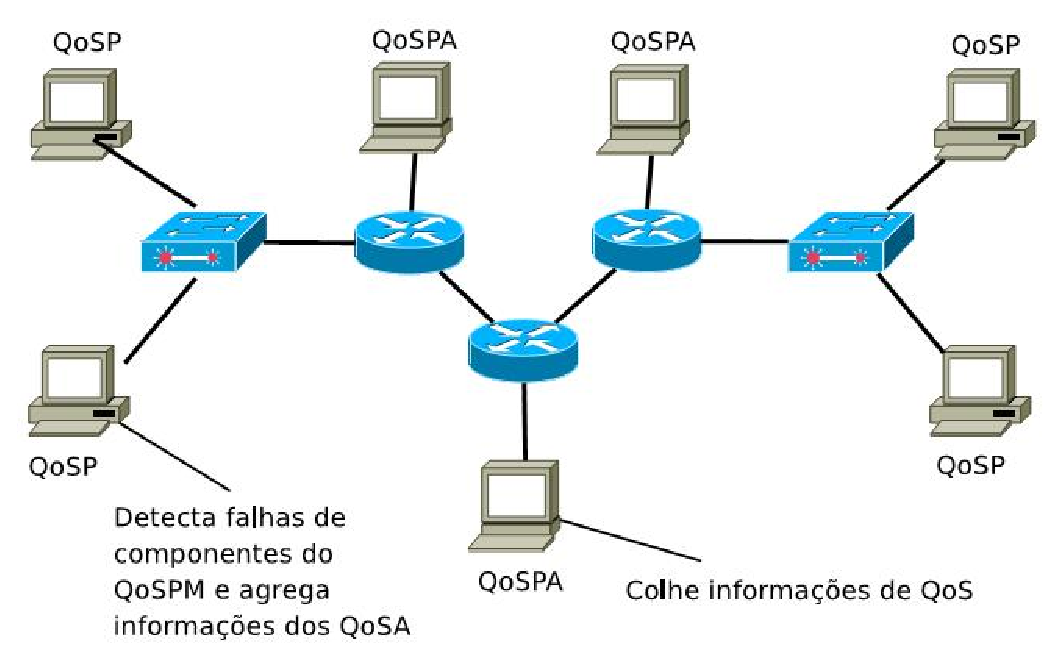
\includegraphics[scale=0.7]{arquitetura_qospm}
\caption{Arquitetura do QoSPM}
\label{fig:arquitetura_qosp}
\end{figure}

\subsection{O QoSP}
	Os módulos do QoSP executam nos \textit{hosts}, sendo que estes \textit{hosts} são aqueles onde se localizam os componentes que caracterizam o modelo HA, assim como os processos distribuídos que executam sobre o modelo HA. Além dos módulos do QoSP trocarem mensagens entre si (como mensagens de requisição remota de verificação de canal), um determinado QoSP comunica-se com vários módulos do QoSPA para colher informações sobre a QoS que está sendo provida para um determinado canal (mas especificadamente para uma determinada classe de serviço da arquitetura Diffserv), cujos roteadores estão sendo monitorados pelos módulos do QoSPA com os quais a comunicação foi estabelecida. Depois de agregada as informações, a QoS do canal pode ser então descoberta. O QoSP também se comunica com o QoSPA para informar sobre seu interesse em receber informações relativas à degradação da QoS no roteador monitorado pelo QoSPA, com o intuito de antecipar o \textit{feedback} provido pelo mecanismo de monitoramento aos processos aplicativos. Sendo assim, a política de notificação de eventos é adotada (ver \ref{cap:qos}).
	
	A arquitetura utilizada pelo QoSP segue a abordagem distribuída adotada pelo modelo de monitoramento descrito no capítulo \ref{cap:qos}. Os componentes \textit{Monitoring Application} e \textit{QoS Monitoring} do modelo de monitoramento fazem parte do QoSP. Além das funções descritas anteriormente, o QoSP é responsável pela detecção de falhas dos elementos que são importantes para o funcionamento do QoSPM (roteadores, módulos do QoSP e módulos do QoSPA).
	
\subsection{O QoSPA}
	Cada módulo do QoSPA está vinculado a um roteador específico e sua função é colher informações sobre QoS no roteador vinculado ao mesmo. O QoSPA executa em um \textit{host} conectado diretamente ao roteador, seguindo um dos princípios de sistemas de monitoramento. Caso o QoSPA não possa executar em \textit{host} específico, o mesmo poderá executar em um \textit{host} onde se localiza um módulo do QoSP. O QoSPA colhe periodicamente informações de QoS, pré-processa e sumariza estas informações que serão utilizadas pelos módulos do QoSP. Neste contexto, o QoSPA funciona como um agente para o QoSP. O componente \textit{Monitor} do modelo de monitoramento faz parte do QoSPA. Seguindo os princípios de sistemas de monitoramento, o QoSPA executa distribuído (um para cada roteador), além das informações colhidas pelos mesmos serem no nível do agregado (no nível das classes do \textit{Diffserv}).
	
	O protocolo utilizado pelo QoSPA para colher informações de QoS é o SNMP. Uma das vantagens de se utilizar o SNMP é que dependendo da granularidade proporcionada pela MIB utilizada para obter informações de QoS, quanto mais específicas forem as variáveis definidas na MIB, menos mensagens serão trocadas entre o QoSPA e o roteador para se obter uma informação mais robusta. O QoSPA utiliza o SNMP para verificar se a QoS que havia sido previamente negociada para um canal continua sendo provida, verificando se a classe Serviço Expresso configurada no roteador continua provendo seus serviços da maneira esperada. Caso seja percebido que ocorreu degradação, todos os módulos do QoSP interessados em receber tal informação serão notificados.
	
\section{Modelagem do QoSPM}
	A especificação do QoSPM foi feita através da modelagem do sistema utilizando a abordagem orientada à objetos, sendo que tal modelagem foi feita utilizando-se a UML \cite{UML99}. Com a modelagem, além de ser possível especificar a estrutura e comportamento do sistema, as decisões tomadas são documentadas \cite{UML99}.
	
	Baseado na arquitetura descrita na seção anterior e na funcionalidade provida pelo mecanismo de monitoramento, a estrutura do QoSPM foi especificada através de diagramas de classe. Foram desenvolvidos diagramas de classe para modelar tanto o QoSP como o QoSPA.
	
\subsection{QoSP}
	Por ser o módulo principal, o QoSP envolveu tanto a modelagem do domínio como a modelagem da aplicação. O domínio representa o vocabulário inerente ao mecanismo de monitoramento do QoS \textit{Provider}. As informações do vocubulário que necessitam serem armazenadas são relativas aos canais de comunicação. O modelo de classes do domínio (Figura \ref{fig:diagrama_classe_dominio}) é formado pelas seguintes entidades:
	
\begin{figure}
\centering
%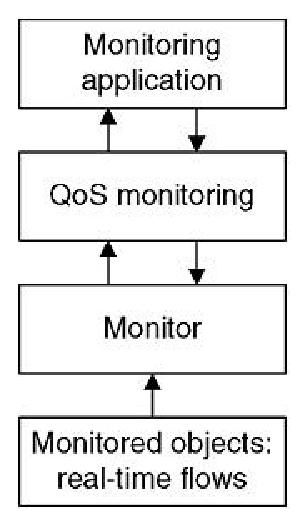
\includegraphics[width=0.3\textwidth]{modelo}
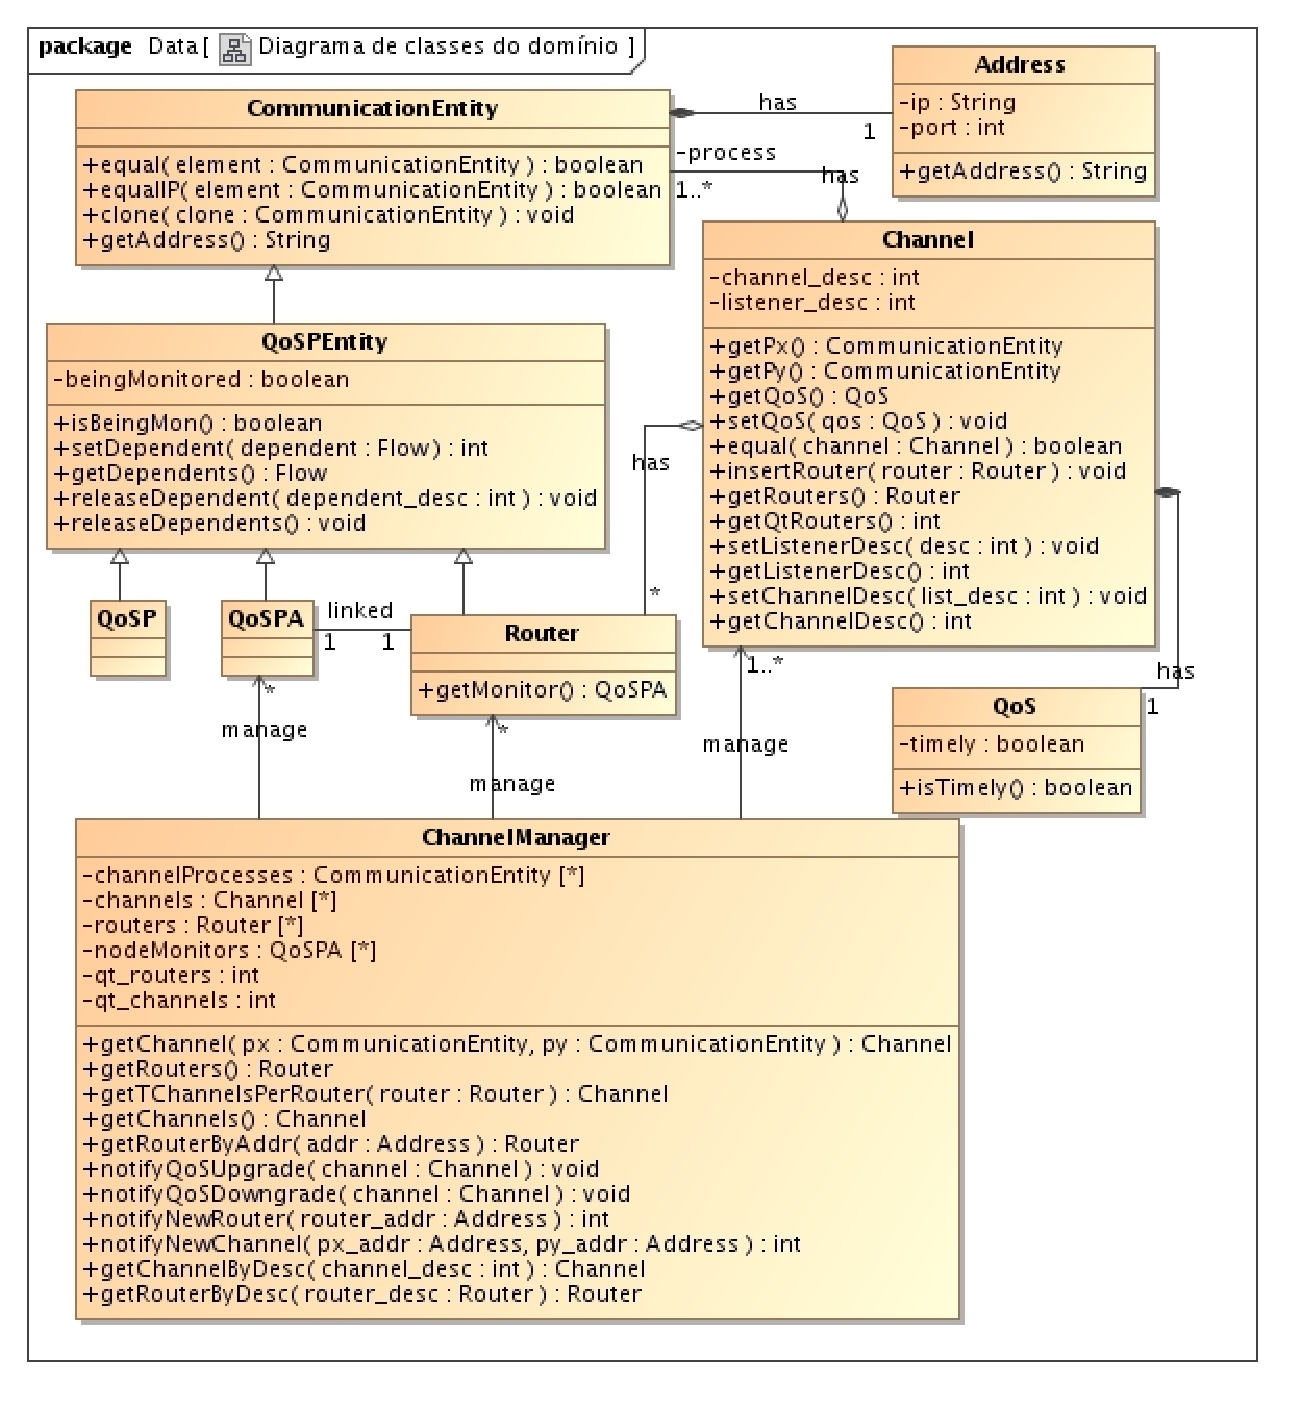
\includegraphics[scale=0.7]{diagrama_dominio}
\caption{Diagrama de classes do Domínio}
\label{fig:diagrama_classe_dominio}
\end{figure}
	
\begin{itemize}
\item \textbf{CommunicationEntity}: Representa qualquer entidade com a qual se possa estabelecer uma comunicação na rede. Essa entidade pode ser tanto um componente de \textit{software} como um componente de \textit{hardware}. Para que essa comunicação seja possível, essa entidade necessita ser localizada através de um endereço IP.

\item \textbf{Address}: Representa um endereço IP de uma \textit{CommunicationEntity}.

\item \textbf{QoSPEntity}: Limita o escopo do que uma \textit{CommunicationEntity} pode ser, mas especificadamente, especifica as entidades que compõem o QoSPM e que, possivelmente, necessitarão ser monitoradas.

\item \textbf{QoSP}: Representa um módulo do QoSP.

\item \textbf{QoSPA}: Representa um módulo do QoSPA.

\item \textbf{Router}: Representa um roteador.

\item \textbf{Channel}: Representa um canal lógico, formado por dois processos e por roteadores.

\item \textbf{QoS}: Representa a QoS de um \textit{Channel}. No contexto do QoSPM, a QoS de um canal só pode ser \textit{TIMELY} ou \textit{UNTIMELY}.

\item \textbf{ChannelManager}: Gerencia o principal recurso do QoS \textit{Provider}, os canais, além dos componentes do QoSPM cujas informações necessitam serem recuperadas pelas classes do modelo de aplicação. É importante salientar que \textit{ChannelManager} gerencia apenas os recursos que, de certa forma, estão relacionados aos canais de comunicação cujos processos localizam-se em seu \textit{host}.	
\end{itemize}
	
	O modelo de aplicação define a aplicação (mecanismo de monitoramento) propriamente dita, e não os objetos (definidos no modelo de domínio) sobre os quais a aplicação atua \cite{BLAHUM06}. A maioria das classes deste modelo são orientadas a computação, diferentemente do modelo de domínio. O modelo de classes da aplicação (Figura \ref{fig:diagrama_classe_qosp}) é formado pelas seguintes entidades:
	
\begin{figure}
\centering
%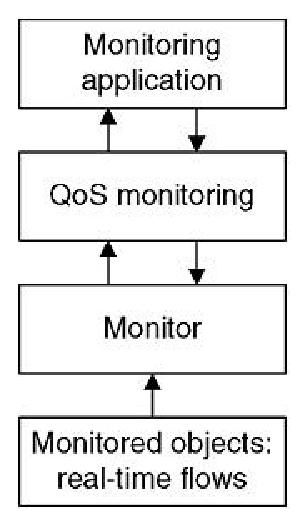
\includegraphics[width=0.3\textwidth]{modelo}
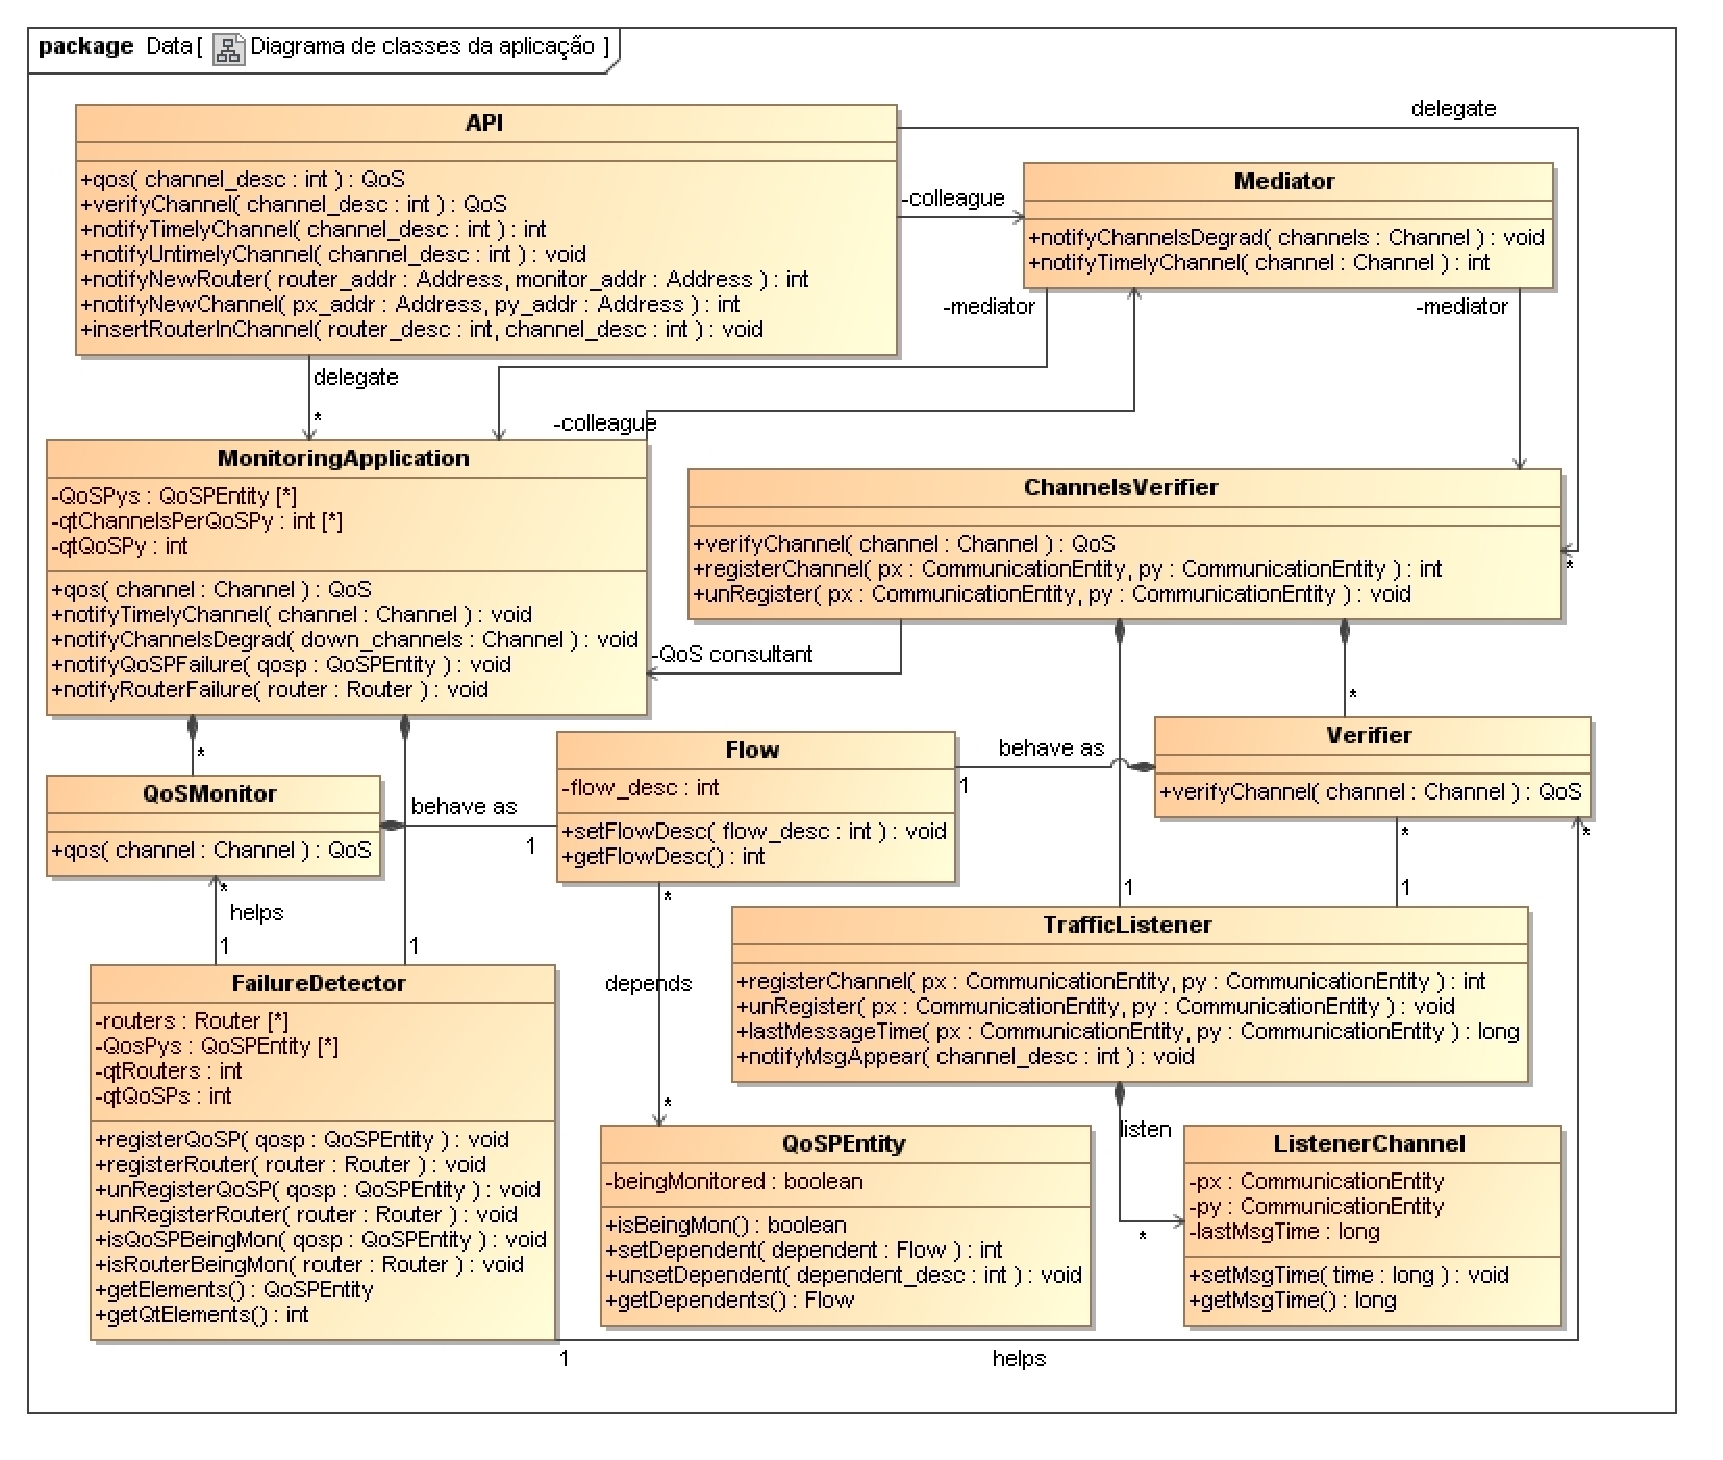
\includegraphics[scale=0.65]{diagrama_aplicacao}
\caption{Diagrama de classes do QoSP}
\label{fig:diagrama_classe_qosp}
\end{figure}	
	
\begin{itemize}
\item \textbf{API}: Representa a interface do QoSPM. Como foi descrito no capítulo \ref{cap:qos_provider}, tanto os processos aplicativos como o módulo de negociação necessitam interagir com o QoSPM. Ambos enxergam o QoSPM através desta classe.

\item \textbf{Mediator}: Encapsula como os objetos das classes \textit{API}, \textit{MonitoringApplication} e \textit{ChannelVerifier} interagem quando há altereção de QoS de um canal. Esta classe modela o principal participante do padrão de projeto \textit{Mediator} \cite{GAHEJOVLI97}.

\item \textbf{MonitoringApplication}: É responsável por delegar cada monitoração de QoS para um \textit{QoSMonitor}. Além disso ela também é responsável por verificar quando um determinado módulo do QoSP não necessita mais ser monitorado pelo \textit{FailureDetector}, visto que não existem mais canais passando pelo \textit{host} do mesmo.

\item \textbf{QoSMonitor}: É responsável por monitorar a QoS de um canal, quando tal monitoramento é requisitado.

\item \textbf{FailureDetector}: Responsável por monitorar periodicamente objetos \textit{QoSPEntity} à procura de falhas. Caso falhas sejam detectadas, objetos \textit{QoSMonitor} assim como objetos \textit{Verifier} podem usufruir de tal informação, visto que, possivelmente, respostas das mensagens enviadas pelos mesmos não chegarão. É importante salientar que \textit{FailureDetector} é a única classe que necessita estabelecer \textit{timeouts} para a recepção de respostas às suas mensagens enviadas. Tanto \textit{QoSMonitor} como \textit{Verifier} não necessitam estabelecer \textit{timeouts} para a execução de suas funções, visto que eles contam com informações providas por \textit{FailureDetector} sobre falhas em componentes que impediriam suas respostas de chegarem.

\item \textbf{ChannelVerifier}: É responsável por delegar cada verificação de canal para um \textit{Verifier}. Além disso ela também é responsável por informar \textit{TrafficListener} quando canais de comunicação devem ou não ser escutados.

\item \textbf{Verifier}: É responsável por realizar a verificação de canal (descrita no capítulo \ref{cap:qos_provider}), quando tal verificação é requisitada.

\item \textbf{TrafficListener}: Responsável por escutar os canais de comunicação e armazenar informações sobre o momento em que houve tráfego nestes canais.

\item \textbf{ListenerChannel}: Representa um canal de comunicação que está sendo escutado por \textit{TrafficListener}.

\item \textbf{Flow}: Modela o comportamento de um fluxo de execução. Tanto \textit{QoSMonitor} como \textit{Verifier} se comportam como um fluxo de execução, visto que tanto a função de monitoração de QoS como a função de verificação de canal podem ter mais de uma requisição sendo realizada ao mesmo tempo.

\end{itemize}

\subsection{QoSPA}

	O módulo do QoSPA tem uma funcionalidade bem mais restrita se comparado ao módulo do QoSP. O diagrama de classes (Figura \ref{fig:diagrama_classe_qospa}) do mesmo é bem simples, sendo formado pelas seguintes classes:
	
\begin{figure}
\centering
%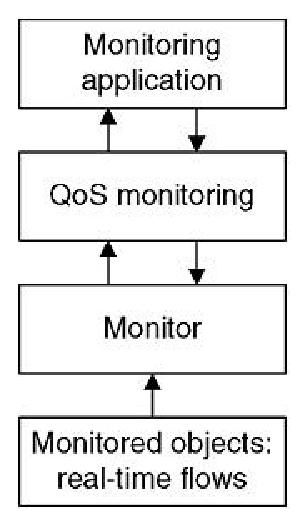
\includegraphics[width=0.3\textwidth]{modelo}
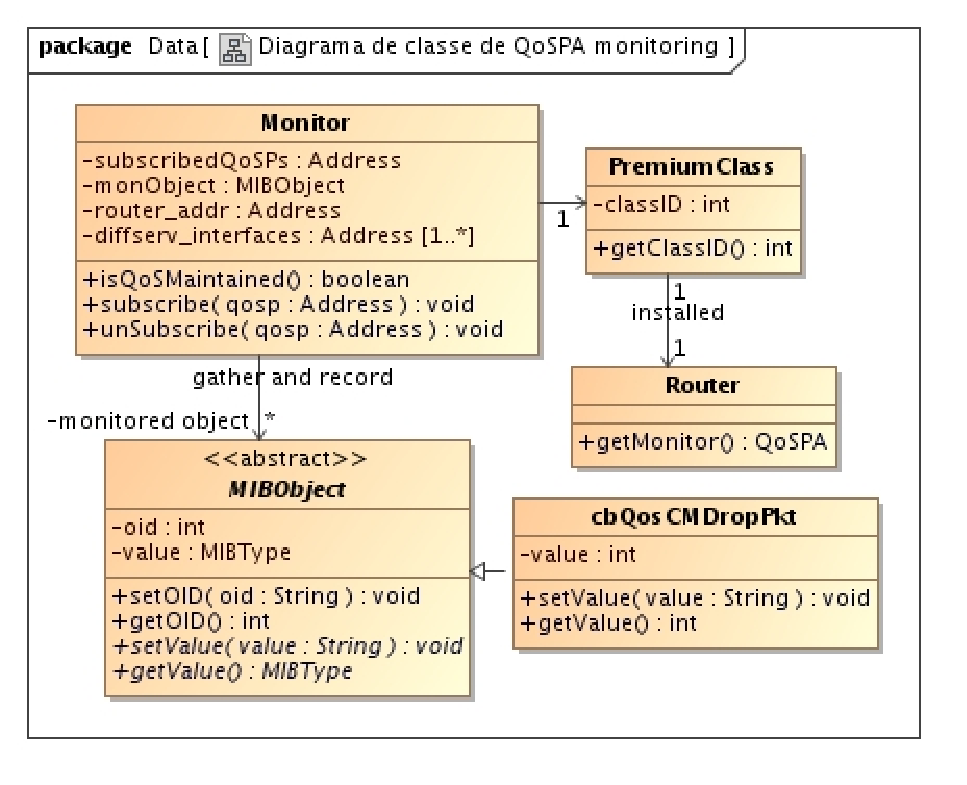
\includegraphics[scale=0.7]{diagrama_qospa}
\caption{Diagrama de classes do QoSPA}
\label{fig:diagrama_classe_qospa}
\end{figure}

\begin{itemize}
\item \textbf{Monitor}: É responsável por colher informações, provenientes do roteador vinculado ao módulo QoSPA do qual faz parte, relativas à classe do serviço Expresso. Essas informações serão utilizadas para verificar se a QoS anteriormente negociada continua sendo provida. Essas informações colhidas correspondem aos \textit{MIBObject}s.

\item \textbf{MIBObject}: Representa um objeto MIB (explicado na seção que descreve o SNMP no capítulo \ref{cap:qos}) colhido por \textit{Monitor}. Cada \textit{MIBObject} corresponde a um \textit{Monitored object} do modelo conceitual de monitoramento (descrito no capítulo \ref{cap:qos}). Essa classe é abstrata pois o tipo do valor de cada objeto MIB pode variar. O objeto MIB capturado deve implementar os métodos abstratos desta classe.

\item \textbf{PremiumClass}: Representa a classe de serviço expresso configurada em um roteador.
\end{itemize}

\section{Protocolo utilizado pelo QoSPM}
	Como foi descrito nas seções anteriores, o QoSPM é composto por módulos do QoSP e do QoSPA que trocam mensagens entre si e com os roteadores. Para descrever tais mensagens, foi definido um protocolo de comunicação. A seguir serão descritas as mensagens que fazem parte do protocolo, sendo que para cada mensagem serão descritos o componente que enviou tal mensagem, o componente receptor, em qual contexto assim como a semântica da mensagem enviada, os campos que compõem a mensagem (toda mensagem possui um campo que identifique o tipo da mensagem, sendo assim este não será citado) e, se houver a necessidade, a ordem de precedência com relação a outras mensagens. A palavra \textit{QoSP} será utilizada de forma intercambiável com a expressão \textit{módulo do QoSP} assim como a palavra \textit{QoSPA} será utilizada de forma intercambiável com a expressão \textit{módulo do QoSPA}, ambos os módulos descritos na seção inicial deste capítulo.
	
\begin{itemize}
\item \textbf{Monitoring Request}: Esta mensagem é enviada por um QoSP para um QoSPA quando uma requisição de monitoramento (função \textit{QoS} descrita no capítulo \ref{cap:qos_provider}) de QoS é executada. Requisita ao QoSPA que verifique junto ao roteador vinculado ao mesmo se a classe Serviço Expresso configurada neste roteador continua provendo seus serviços da maneira esperada. Tal mensagem possui um campo que identifica uma requisição de monitoramento específica, visto que várias requisições de monitoramento podem ser feitas ao mesmo tempo. Além disso, ela possui um campo que identifica unicamente uma mensagem deste tipo, visando descartar mensagens antigas.

\item \textbf{Monitoring Reply}: Esta mensagem é enviada por um QoSPA para um QoSP em resposta à mensagem \textit{Monitoring Request} previamente enviada. Depois que QoSPA verifica junto ao roteador vinculado ao mesmo se a classe Serviço Expresso configurada neste roteador continua provendo seus serviços da maneira esperada, ele manda a resposta ao QoSP. Tal mensagem possui um campo que informa se a QoS está mantida, além de dois outros campos cujos valores e tipos são os mesmos da mensagem \textit{Monitoring Request} recebida.

\item \textbf{Monitoring Reply Ack.}: Esta mensagem é enviada por um QoSP para um QoSPA em resposta à mensagem \textit{Monitoring Reply} previamente recebida, sendo que na mensagem \textit{Monitoring Reply} consta que houve degradação da QoS. Depois que o QoSP recebeu do QoSPA a resposta do monitoramento e descobriu que houve degradação, ele deve enviar uma mensagem de reconhecimento. Isto é importante pois como ocorreu degradação, a resposta do monitoramento pode não ter sido entregue ao QoSP. Tal mensagem possui dois campos cujos valores e tipos são os mesmos dos dois últimos campos de \textit{Monitoring Reply}.

\item \textbf{Verification Request}: Esta mensagem é enviada por um QoSP para outro QoSP quando uma requisição de verificação de canal (função \textit{Verify Channel} descrita no capítulo \ref{cap:qos_provider}) é executada, sendo que o canal em questão não é gerenciado pelo QoSP local (uma requisição remota deve ser executada). Tal mensagem requisita ao QoSP remoto que faça uma verificação local do canal em questão. Tal mensagem possui um campo que identifica os dois processos (através dos endereços IP) que fazem parte do canal a ser verificado. Além disso, esta mensagem possui dois outros campos semelhantes aos campos  de \textit{Monitoring Request}.

\item \textbf{Verification Reply}: Esta mensagem é enviada por um QoSP para outro QoSP em resposta à mensagem \textit{Verification Request} previamente enviada. Depois que o QoSP verifica localmente um canal (através da execução da função \textit{Verify Channel}), ele manda a resposta ao QoSP que havia solicitado a verificação remota. Tal mensagem possui um campo com o resultado da verificação local, além de dois outros campos cujos valores e tipos são os mesmos dos dois últimos campos de \textit{Verification Request}.

\item \textbf{Subscribe}: Esta mensagem é enviada por um QoSP para um QoSPA quando um canal teve sua QoS alterada para \textit{TIMELY}, sendo que o QoSPA em questão ainda não havia recebido tal mensagem anteriormente. O QoSP envia tal mensagem ao QoSPA para informar que está interessado em receber informações sobre degradação da QoS provida pelo roteador no qual o QoSPA está vinculado. O intuito desta mensagem é de antecipar a informação sobre degradação da QoS, consequentemente antecipar o \textit{feedback} provido pelo QoSPM. Esta mensagem não possui nenhum campo adicional.

\item \textbf{Unsubscribe}: Esta mensagem é enviada por um QoSP para um QoSPA quando a QoS de todos os canais, que passam pelo roteador vinculado ao QoSPA em questão e que são gerenciados pelo QoSP, foi rebaixada para \textit{UNTIMELY}. O QoSP envia tal mensagem ao QoSPA para informar que não está mais interessado em receber informações sobre degradação da QoS provida pelo roteador no qual o QoSPA está vinculado. Esta mensagem não possui nenhum campo adicional.

\item \textbf{Notify Degradation}: Esta mensagem é enviada por um QoSPA para um(ns) QoSP(s) quando, depois que informações de QoS são colhidas e pré-processadas, percebe-se que houve degradação da QoS provida pelo roteador. Tal mensagem é enviada para todos os QoSPs que estão interessados em receber informação de degradação de QoS no roteador vinculado ao QoSPA em questão. Esta mensagem não possui nenhum campo adicional.

\item \textbf{Are you alive}: Esta mensagem é enviada por um QoSP (mas especificadamente pelo detector de falhas do QoSP) para um QoSP/QoSPA/roteador periodicamente. Tal mensagem tem por objetivo verificar se um determinado componente do QoSPM falhou. Esta mensagem equivale a um \textit{Echo Request} do protocolo ICMP. Possui um campo que identifica unicamente uma mensagem deste tipo, além de um campo que identifica o elemento (QoSP ou QoSPA ou roteador) para o qual está sendo enviada a mensagem. Este campo é necessário para que o detector de falhas possa saber quais os elementos que responderam a esta mensagem dentro do limite temporal.

\item \textbf{Explicit ping}: Esta mensagem é semelhante à \textit{Are you alive}, mas ela é enviada para um QoSP quando uma requisição de monitoramento de QoS é executada. O QoSP para o qual a mensagem é enviada localiza-se no mesmo \textit{host} de $p_{y}$, sendo $p_{y}$ o processo remoto do canal cuja monitoração foi solicitada. Esta mensagem, em complemento às mensagens \textit{Monitoring Request} enviadas, são necessárias para a execução do monitoramento de QoS. Esta mensagem não possui um campo que identifica o elemento para o qual a mensagem foi enviada, mas possui um campo que identifa uma requisição de monitoramento específica. 

\item \textbf{I am alive}: Esta mensagem é enviada por um QoSP/QoSPA/roteador para um QoSP em resposta à mensagem \textit{Are you alive} (ou \textit{Explicit ping}) previamente recebida. Ela equivale a um \textit{Echo Reply} do protocolo ICMP. Tal mensagem possui dois campos cujos valores e tipos são os mesmos da mensagem \textit{Are you alive} (ou \textit{Explicit ping}) recebida.
\end{itemize}

	Além das mensagens descritas acima, o QoSPM utiliza mensagens SNMP (estas não fazem parte do protocolo definido visto que o SNMP já é um protocolo padronizado) na sua comunicação. As mensagens SNMP são trocadas entre o QoSPA e o roteador vinculado ao mesmo, e tem por objetivo colher informações de QoS. As seguintes mensagens foram utilizadas:
	
\begin{itemize}
\item \textbf{Get Request}: Enviada por um QoSPA para o roteador vinculado ao mesmo quando o QoSPA deseja verificar se a QoS continua sendo mantida. Esta mensagem é utilizada para capturar o valor de uma ou mais variáveis MIB (descritas no capítulo \ref{cap:qos}).

\item \textbf{Get Response}: Enviada por um roteador para o QoSPA no qual está vinculado em resposta à mensagem \textit{Get Request} previamente recebida. Ela contém os valores das variáveis MIB requisitados.
\end{itemize}	

\section{Algoritmos do QoSPM}

	Para completar o desenvolvimento do QoSPM, os algoritmos que o compõe foram especificados. Para cada algoritmo será descrita sua funcionalidade, assim como o contexto em que o mesmo executa. As mensagens citadas na descrição dos algoritmos são as mesmas descritas na seção anterior. Assim como na seção anterior, a palavra \textit{QoSP} será utilizada de forma intercambiável com a expressão \textit{módulo do QoSP} assim como a palavra \textit{QoSPA} será utilizada de forma intercambiável com a expressão \textit{módulo do QoSPA}.

%macros definidas por mim
\SetKwFor{AtEvery}{At every}{do}{end}
\SetKw{Task}{Task}
\SetKw{Execute}{execute}
\SetKw{Wait}{wait for}
\SetKwFor{When}{when}{do}{end}
%fim

\begin{itemize}
\item \textbf{Failure Detector} (Algoritmo 1): Algoritmo composto por duas tarefas que executam em paralelo no contexto do \textit{Failure Detector} do QoSPM. Tais tarefas são responsáveis por detectar a falha dos componentes do QoSPM, mas especificadamente QoSP, QoSPA e roteadores. É importante ressaltar que cada QoSP monitora apenas os componentes que estão relacionados com os canais gerenciados pelo mesmo. A tarefa \textit{detectFailure} é responsável por enviar periodicamente mensagens \textit{"Are you alive ?"} para os componentes de interesse do QoSP. A periodicidade do monitoramento é definido através do parâmetro \textit{FD monitoring interval}. O vetor \textit{elements} armazena os componentes que devem ser monitorados. A função \textit{getElements()} retorna os elementos que devem ser monitorados ordenados pelo tempo de transferência de mensagens entre o QoSP local e o componente em questão, sendo que este tempo é calculado pela função \textit{Delay}. A variável \textit{ExpectedMsg} identifica o elemento cuja mensagem \textit{"I am alive"} possivelmente será a próxima a ser recebida. Esta variável é compartilhada pelas duas tarefas. O vetor \textit{ReplyStatus} guarda a informação dos elementos cujas mensagens \textit{"I am alive"} já chegaram. Este vetor também é compartilhado pelas duas tarefas. A função \textit{CT()} retorna a hora local. A declaração \textit{Set EventWait(EVENT, timeout)} serve para indicar que a ocorrência de um evento será aguardada ou a ocorrência de um \textit{timeout}, o que vier primeiro. Basicamente, o algoritmo funciona da seguinte maneira: baseado nas mensagens \textit{"I am alive"} que ainda não chegaram, a função \textit{EventWait} configura o \textit{timeout} para o elemento cuja mensagem \textit{"I am alive"} é a próxima esperada. Quando uma determinada mensagem não chegou no tempo esperado, é notificada a falha do componente correspondente. Uma vantagem deste algoritmo é que com apenas uma única \textit{thread} de execução é possível monitorar todos os elementos concorrentemente, sendo que o tempo máximo para executar uma rodada deste algoritmo corresponde ao \textit{delay} calculado para o último elemento do vetor \textit{elements}.

	A tarefa \textit{fdListener} é responsável por ficar escutando o canal do \textit{Failure Detector} e atualizando \textit{ReplyStatus} com as informações dos elementos cujas mensagens \textit{"I am alive"} já chegaram. Além do mais, ela é responsável por sinalizar a chegada da mensagem esperada.
	
\SetAlgoSkip{0em}
\SetAlgoInsideSkip{0em}
\SetAlCapSkip{0em}
\SetVlineSkip{0em}
\setlength{\algomargin}{0em}
%\Setnlskip{0em}
\SetAlFnt{\small}
%\SetDataSty{}
%\SetInd{0em}{0em}
%\SetAlTitleFnt{textit}
%\SetAlFont{\small\em}	
%\begin{algorithm}[H]
\begin{algorithm}[H]
%AlFont{\small\em}
%\dontprintsemicolon
%\SetVline
%\KwData{elements}
%\KwData{ExpectedMsg}
%\KwData{ReplyStatus}
\Task{detectFailure}\;
\Begin{
\AtEvery{FD monitoring interval}{
	%$elements \leftarrow$ FD.getElements()\;
	$elements \leftarrow getElements()$\;
	$ExpectedMsg \leftarrow 1$\;
	\ForEach{$element \in elements$}{
	$ReplyStatus[element] \leftarrow NotReceived$\;
	$AliveMsg.id \leftarrow element$\;
	$MsgSentTime[element] \leftarrow CT()$\;
	send $"AliveMsg"$ message to $element$\;
	}
	
	\textbf{Set} EventWait($ExpectedMsgReceived$, Delay(localQoSP, $elements[1]$))\;
	\ForEach{$element \in elements$}{
		\If{$ReplyStatus[element] = NotReceived$}{
			\If{$element = ExpectedMsg$}{
				\If{$element.type = QoSP$}{
					%FD.notifyQoSPFailure($element$)\;
					$notifyQoSPFailure(element)$\;
				}
				\ElseIf{$element.type = QoSPA$}{
					$notifyQoSPAFailure(element)$\;
				}
				\Else{
					%FD.notifyRouterFailure($element$)\;
					$notifyRouterFailure(element)$\;
				}
				\lIf{element is the last}{$continue$\;}
				$ExpectedMsg \leftarrow ExpectedMsg + 1$\;				
				%\textbf{Set} EventWait($ExpectedMsgReceived$, $MsgSentTime[ExpectedMsg] + Delay(localQoSP, \; elements[ExpectedMsg] - CT()$))\;
			}
			\Else{
				$ExpectedMsg \leftarrow element$\;
				%\textbf{Set} EventWait($ExpectedMsgReceived$, $MsgSentTime[ExpectedMsg] + Delay(localQoSP, elements[ExpectedMsg] - CT()$))\;
			}
			\textbf{Set} EventWait($ExpectedMsgReceived$, $MsgSentTime[ExpectedMsg] + Delay(localQoSP, elements[ExpectedMsg]) - CT()$)\;
		}
	}
}
}

\Task{fdListener}\;
\Begin{
	%\When{AliveMsgReply is received}{
	\textbf{wait for}(receive message $"AliveMsgReply"$)\;
		$ReplyStatus[AliveMsgReply.id] \leftarrow Received$\;
		\If{$ExpectedMsg = AliveMsgReply.id$}{
			SignalEvent($ExpectedMsgReceived$)\;
		}
	%}
}
\caption{Failure Detector}
\end{algorithm}	

\item \textbf{QoS} (Algoritmo 2): Responsável por verificar a QoS que está sendo provida ao canal de comunicação $c_{x/y}$ (equivale à função $QoS(p_{x}, p_{y})$ descrita no capítulo \ref{cap:qos_provider}). Esse algoritmo executa a tarefa \textit{checkQoSP} em paralelo com o resto do algoritmo. A tarefa \textit{checkQoSP} é responsável por verificar se um QoSP está vivo, através do envio da mensagem $"ExplicitPing"$. Caso a resposta não chegue dentro do \textit{timeout}, o resultado da verificação será \textit{UNTIMELY}. Para verificar a QoS do canal $c_{x/y}$, o algoritmo verifica se $QoSP_{y}$ está vivo além de enviar mensagens $"MonitoringRequest"$ para os QoSPA dos roteadores pertencentes ao canal $c_{x/y}$. Se todas as respostas dos QoSPA chegarem, informando que a QoS está mantida, o resultado da verificação é \textit{TIMELY}, caso contrário será \textit{UNTIMELY}. Observe que exceto pela tarefa \textit{checkQoSP}, o algoritmo não estabelece \textit{timeout} para o recebimento das mensagens. Visto que os canais do QoS Provider usufruem dos serviços isócronos, caso as mensagens não cheguem, foi decorrente da falha de um componente do QoSPM, cuja falha será notificada pelo \textit{Failure Detector}.

\begin{algorithm}[H]
	\Task{checkQoSP($QoSP_{y}$)}\;
	\Begin{
		$AliveMsg.id \leftarrow ExplicitPing$\;
		send $"AliveMsg"$ message to $QoSP_{y}$\;
		$timeout \leftarrow CT() + Delay(localQoSP, QoSP_{y})$\;
		%\When{$CT\left(\right) > timeout \vee AliveMsgReply \; is \; received$}{
		%\textbf{wait for}((receive message $AliveMsgReply$ from $QoSP_{y}$) \vee \; ($CT() > timeout$))\;
		\textbf{wait for}($(receive \; message \; AliveMsgReply \; from \; QoSP_{y}) \vee (CT() > timeout)$)\;
		\If{$CT\left(\right) > timeout$}{
			\Return{UNTIMELY}\;
		}
		%}
	}
	
	\Execute{checkQoSP($QoSP_{y}$)}\;
	\ForEach{$router \in channels[c_{x/y}]$}{
		send $"MonitoringRequest"$ message to QoSPA(router)\;
	}
	%\textbf{wait for}(((receive message $MonitoringReply(maintained)$ from QoSPA(router)) \vee \; (router \; has \; failed)) \; $\forall router \in channels[c_{x/y}]$)\;
	\textbf{wait for}($((receive \; message \; MonitoringReply(maintained) \; from \; QoSPA(router)) \vee  (router \vee QoSPA(router) \; has \; failed)) \; \forall router \in channels[c_{x/y}]$)\;
	\If{received every message MonitoringReply(maintained) $\wedge$ \; ($\forall message \; MonitoringReply(maintained), \; maintained = True$)}{
		\Return{TIMELY}\;
	}
	\Else{
		\Return{UNTIMELY}\;
	}
\caption{QoS($p_{x}, p_{y}$)}
\end{algorithm}

\item \textbf{VerifyChannel} (Algoritmo 3): Equivale à função $VerifyChannel(c_{x/y})$ descrita no capítulo três. Caso o canal $c_{x/y}$ não seja gerenciado pelo QoSP local, uma requisição remota será executada atráves do envio da mensagem $"VerificationRequest"$. O resultado da verificação remota será o resultado da função. Assim como no algoritmo $QoS(p_{x}, p_{y})$, não utiliza-se \textit{timeout}. Caso o canal seja gerenciado localmente, o resultado da função será encontrado através da execução da função \textit{QoS}, seguido de uma verificação de tráfego no canal, se necessário. O resultado da função \textit{VerifyChannel} será \textit{TIMELY} se o resultado da execução da função \textit{QoS} for \textit{TIMELY} e logo em seguida for percebido que houve tráfego no canal $c_{x/y}$ durante um certo intervalo de tempo (estabelecido pelo modelo HA). Caso contrário o resultado da função será \textit{UNTIMELY}.

\begin{algorithm}[H]
	\If{$c_{x/y} \notin channels$}{
		send $"VerificationRequest(c_{x/y})"$ message to $QoSP_{x}$\;
		\textbf{wait for}((received message $VerificationReply(c_{x/y},qos)$ from $QoSP_{x}$) $\vee$ \; ($QoSP_{x}$ has failed))\;
		\If{$received \; message \; VerificationReply(c_{x/y}, \; qos) \wedge qos = TIMELY$}{
			\Return{TIMELY}\;
		}
		\Else{
			\Return{UNTIMELY}\;
		}
	}
	\Else{
		$qos \leftarrow QoS(p_{x}, p_{y})$\;
		\If{$qos = UNTIMELY$}{
			\Return{UNTIMELY}\;
		}
		\Else{
			$starttime \leftarrow CT()$\;
			$timeout \leftarrow \textit{CHANNEL\_DORMANCY\_PERIOD}$\;
			\textbf{wait for}($CT() > timeout$)\;
			%\If{$TrafficListener.lastMessageTime(p_{x}, p_{y}) < starttime$}{
			\If{$lastMessageTime(p_{x}, p_{y}) < starttime$}{
				\Return{UNTIMELY}\;
			}
			\Else{
				\Return{TIMELY}\;
			}
		}
	}
\caption{VerifyChannel($c_{x/y}$)}
\end{algorithm}

\item \textbf{notifyTimelyChannel} (Algoritmo 4): Representa a função que é chamada para notificar que a QoS de um canal ($c_{x/y}$) foi alterada para \textit{TIMELY}. Informa aos QoSPA dos roteadores que compõem o canal $c_{x/y}$, para os quais este procedimento ainda não foi realizado, seu interesse em receber notificação de degradação. Além disso, registra os roteadores e o $QoSP_{y}$, ambos se necessário, junto ao \textit{Failure Detector} para monitorá-los. Finaliza registrando o canal formado pelos processos $p_{x}$ e $p_{y}$ junto ao \textit{Traffic Listener} (descrito na modelagem do QoSPM).

\begin{algorithm}[H]
	\ForEach{$router \in channels[c_{x/y}]$}{
		\If{$QoSP_{x}$ is not subscribed with QoSPA(router)}{
			send $"Subscribe"$ message to QoSPA(router)\;
		}
		\If{router is not being monitored by FailureDetector}{
			%FailureDetector.registerRouter(router)\;
			\textbf{Set} \textit{Failure Detector} to monitor $router$\;
		}
	}
	\If{$QoSP_{y}$ is not being monitored by FailureDetector}{
		%FailureDetector.registerQoSP($QoSP_{y}$)\;
		\textbf{Set} \textit{Failure Detector} to monitor $QoSP_{y}$\;
	}
	%TrafficListener.registerChannel($p_{x}$, $p_{y}$)\;
	register $channels[c_{x/y}]$ with \textit{Traffic Listener}\;
\caption{notifyTimelyChannel($p_{x}, p_{y}$)}
\end{algorithm}

\item \textbf{notifyChannelsDegradation} (Algoritmo 5): Representa a função que é chamada para informar que um conjunto de canais teve sua QoS degradada para \textit{UNTIMELY}. A degradação pode ter sido decorrente à notificação de falha (por parte de \textit{Failure Detector}) de um QoSPA ou roteador ou de um QoSP, ou decorrente à notificação (por parte do QoSPA) de que um roteador não está podendo prover um serviço previamente negociado, ou ainda decorrente à notificação (por parte do mecanismo de admissão) de que a QoS de um canal de comunicação foi rebaixada para \textit{UNTIMELY}. Basicamente esse algoritmo realiza o procedimento inverso do algoritmo anterior, cancelando os registros dos elementos que não necessitam serem mais monitorados (em contextos diferentes, dependendo do elemento).

\begin{algorithm}[H]
	\ForEach{$c_{x/y} \in downChannels$}{
		%$channels_{y}$ \leftarrow $\left\lbrace aux_{x/d}$ | $aux_{x/d} \in channels$ and $d = y$ \right\rbrace\;
		%$channels_{y} \leftarrow$ \left\lbrace $aux_{x/d}$ | $aux_{x/d} \in channels$ {\bf and} $d = y$ \right\rbrace\;\
		$channels_{y} \leftarrow \left\lbrace aux_{x/d} | \left( aux_{x/d} \in channels \right) \wedge \left( d = y \right) \right\rbrace$\;
		\If{$\left\lbrace c_{x/y} \right\rbrace = channels_{y}$ }{
			%FailureDetector.unRegisterQoSP($QoSP_{y}$)\;
			\textbf{unSet} \textit{Failure Detector} to monitor $QoSP_{y}$\;
		}
		%TrafficListener.unRegister($p_{x}$, $p_{y}$)\;
		unRegister $channels[c_{x/y}]$ with \textit{Traffic Listener}\;
		notify $p_{x}$ about $c_{x/y}$ degradation\;
	}
	
	\ForEach{router managed by QoSP}{
		%routedChannels \leftarrow \left\lbrace aux_{x/y} | $aux_{x/y} \in channels$ {\bf and} $router \in aux_{x/y}$ \right\rbrace \;
		$routedChannels \leftarrow \left\lbrace aux_{x/y} | \left( aux_{x/y} \in channels \right) \wedge \left( router \in aux_{x/y} \right) \right\rbrace$ \;
		\If{$routedChannels \subseteq downChannels$}{
			%FailureDetector.unRegisterRouter(router)\;
			\textbf{unSet} \textit{Failure Detector} to monitor $router$\;
			send $"unSubscribe"$ message to QoSPA(router)\;
		}
	}
\caption{notifyChannelsDegradation(downChannels)}
\end{algorithm}

\item \textbf{isQoSMaintained} (Algoritmo 6): Representa a função que será utilizada pelo QoSPA para verificar se a QoS contratada para os canais de comunicação \textit{TIMELY} que passam pelo roteador monitorado pelo mesmo continua sendo provida. As mensagens $"GetRequest"$ e $"GetResponse"$ fazem do protocolo SNMP e são utilizadas para capturar o valor de uma variável MIB ($oid$). Quando observa-se que a QoS fornecida pelo roteador foi degradada, o QoSPA envia a mensagem $"Degradation"$ para todos os QoSP que estão interessados em receber tal informação. Esta função também é chamada periodicamente para que o monitoramento automático do roteador possa ocorrer.

\begin{algorithm}[H]
	send $"GetRequest(oid)"$ message to router\;
	\textbf{wait for}($(receive \; message \; GetResponse(oid) \; from \; router)$)\;
	$result \leftarrow ProcessOID(oid)$\;
	\If{$result \neq MAINTAINED$}{
		\ForEach{QoSP subscribed}{
			send $"Degradation"$ message to QoSP\;
		}
		\Return{False}\;
	}
	\Else{
		\Return{True}\;
	}
\caption{isQoSMaintained()}
\end{algorithm}
\end{itemize}

	As tarefas mencionadas nas descrições dos algoritmos (\textit{detectFailure}, \textit{fdListener} e \textit{checkQoSP}) necessitam ser de tempo real para executar suas funções corretamente. Iste se deve ao fato das mesmas estabelecerem \textit{timeout} para a execução de suas funções.